\paragraph{Aclaración} En todos los desarrollos estamos asumiendo que vale el modelo linealizado del PLL. Si no tenés idea de que significa esto, leete las notas de Cioffi\cite{Cio6}.

\section{Ejercicio 1 - PLL de primer orden}
Considere un sistema de recuperación de portadora que utiliza un PLL. Asuma que el error de fase es lo suficientemente pequeño como para que el modelo lineal del PLL dado por la Figura 1 sea aceptable. Asuma que el filtro de lazo L(s) tiene una transferencia de orden cero L(s) = K.

\subsection{Item 1}\paragraph{Enunciado}Determine la transferencia del sistema a lazo cerrado: \[G(s) = \frac{\hat{\Theta}(s)}{\Theta(s)}\] y la transferencia del error: \[G_e(s)=\frac{E(s)}{\Theta(s)}\] determinando los valores de K para los cuales el lazo es estable.

\begin{figure}[h]
	\centering
	% Graphic for TeX using PGF
% Creator: Dia v0.97.2
% CreationDate: Thu Jan 22 22:36:39 2015
% For: Fernando Danko
% \usepackage{tikz}
% The following commands are not supported in PSTricks at present
% We define them conditionally, so when they are implemented,
% this pgf file will use them.
%
% El código producido por DIA fue modificado a mano para mejorar el aspecto.
% Cambios:
% * Las etiquetas se pasaron a LaTeX. Se aumentó el tamaño con \huge{$ec$}
% y con \LARGE{$ec$}.
% * Se movieron las posiciones de las etiquetas

\ifx\du\undefined
  \newlength{\du}
\fi
\setlength{\du}{15\unitlength}
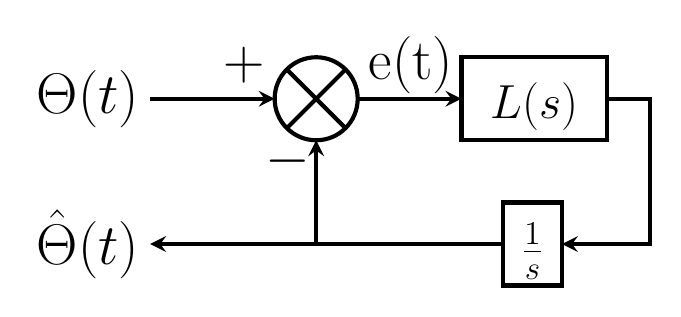
\begin{tikzpicture}
\pgftransformxscale{1.000000}
\pgftransformyscale{-1.000000}
\definecolor{dialinecolor}{rgb}{0.000000, 0.000000, 0.000000}
\pgfsetstrokecolor{dialinecolor}
\definecolor{dialinecolor}{rgb}{1.000000, 1.000000, 1.000000}
\pgfsetfillcolor{dialinecolor}
\definecolor{dialinecolor}{rgb}{1.000000, 1.000000, 1.000000}
\pgfsetfillcolor{dialinecolor}
\fill (12.500000\du,6.000000\du)--(12.500000\du,8.000000\du)--(16.000000\du,8.000000\du)--(16.000000\du,6.000000\du)--cycle;
\pgfsetlinewidth{0.100000\du}
\pgfsetdash{}{0pt}
\pgfsetdash{}{0pt}
\pgfsetmiterjoin
\definecolor{dialinecolor}{rgb}{0.000000, 0.000000, 0.000000}
\pgfsetstrokecolor{dialinecolor}
\draw (12.500000\du,6.000000\du)--(12.500000\du,8.000000\du)--(16.000000\du,8.000000\du)--(16.000000\du,6.000000\du)--cycle;
% setfont left to latex
\definecolor{dialinecolor}{rgb}{0.000000, 0.000000, 0.000000}
\pgfsetstrokecolor{dialinecolor}
\node at (14.250000\du,7.180000\du){\LARGE{$L(s)$}};
\definecolor{dialinecolor}{rgb}{1.000000, 1.000000, 1.000000}
\pgfsetfillcolor{dialinecolor}
\fill (13.500000\du,9.500000\du)--(13.500000\du,11.500000\du)--(14.920000\du,11.500000\du)--(14.920000\du,9.500000\du)--cycle;
\pgfsetlinewidth{0.100000\du}
\pgfsetdash{}{0pt}
\pgfsetdash{}{0pt}
\pgfsetmiterjoin
\definecolor{dialinecolor}{rgb}{0.000000, 0.000000, 0.000000}
\pgfsetstrokecolor{dialinecolor}
\draw (13.500000\du,9.500000\du)--(13.500000\du,11.500000\du)--(14.920000\du,11.500000\du)--(14.920000\du,9.500000\du)--cycle;
% setfont left to latex
\definecolor{dialinecolor}{rgb}{0.000000, 0.000000, 0.000000}
\pgfsetstrokecolor{dialinecolor}
\node at (14.210000\du,10.680000\du){\LARGE{$\frac{1}{s}$}};
\pgfsetlinewidth{0.100000\du}
\pgfsetdash{}{0pt}
\pgfsetdash{}{0pt}
\pgfsetmiterjoin
\pgfsetbuttcap
{
\definecolor{dialinecolor}{rgb}{0.000000, 0.000000, 0.000000}
\pgfsetfillcolor{dialinecolor}
% was here!!!
\pgfsetarrowsend{stealth}
{\pgfsetcornersarced{\pgfpoint{0.000000\du}{0.000000\du}}\definecolor{dialinecolor}{rgb}{0.000000, 0.000000, 0.000000}
\pgfsetstrokecolor{dialinecolor}
\draw (16.000000\du,7.000000\du)--(17.050000\du,7.000000\du)--(17.050000\du,10.500000\du)--(14.920000\du,10.500000\du);
}}
% setfont left to latex
\definecolor{dialinecolor}{rgb}{0.000000, 0.000000, 0.000000}
\pgfsetstrokecolor{dialinecolor}
\node[anchor=west] at (2.000000\du,7.000000\du){\huge{$\Theta(t)$}};
% setfont left to latex
\definecolor{dialinecolor}{rgb}{0.000000, 0.000000, 0.000000}
\pgfsetstrokecolor{dialinecolor}
\node[anchor=west] at (2.000000\du,10.500000\du){\huge{$\hat{\Theta}(t)$}};
\pgfsetlinewidth{0.100000\du}
\pgfsetdash{}{0pt}
\pgfsetdash{}{0pt}
\pgfsetbuttcap
{
\definecolor{dialinecolor}{rgb}{0.000000, 0.000000, 0.000000}
\pgfsetfillcolor{dialinecolor}
% was here!!!
\pgfsetarrowsend{stealth}
\definecolor{dialinecolor}{rgb}{0.000000, 0.000000, 0.000000}
\pgfsetstrokecolor{dialinecolor}
\draw (10.000000\du,7.000000\du)--(12.500000\du,7.000000\du);
}
% setfont left to latex
\definecolor{dialinecolor}{rgb}{0.000000, 0.000000, 0.000000}
\pgfsetstrokecolor{dialinecolor}
\node[anchor=west] at (14.210000\du,10.500000\du){};
\pgfsetlinewidth{0.100000\du}
\pgfsetdash{}{0pt}
\pgfsetdash{}{0pt}
\pgfsetbuttcap
{
\definecolor{dialinecolor}{rgb}{0.000000, 0.000000, 0.000000}
\pgfsetfillcolor{dialinecolor}
% was here!!!
\pgfsetarrowsend{stealth}
\definecolor{dialinecolor}{rgb}{0.000000, 0.000000, 0.000000}
\pgfsetstrokecolor{dialinecolor}
\draw (13.500000\du,10.500000\du)--(5.000000\du,10.500000\du);
}
\pgfsetlinewidth{0.100000\du}
\pgfsetdash{}{0pt}
\pgfsetdash{}{0pt}
\pgfsetbuttcap
{
\definecolor{dialinecolor}{rgb}{0.000000, 0.000000, 0.000000}
\pgfsetfillcolor{dialinecolor}
% was here!!!
\pgfsetarrowsend{stealth}
\definecolor{dialinecolor}{rgb}{0.000000, 0.000000, 0.000000}
\pgfsetstrokecolor{dialinecolor}
\draw (9.000000\du,10.500000\du)--(9.000000\du,8.000000\du);
}
\pgfsetlinewidth{0.100000\du}
\pgfsetdash{}{0pt}
\pgfsetdash{}{0pt}
\pgfsetbuttcap
{
\definecolor{dialinecolor}{rgb}{0.000000, 0.000000, 0.000000}
\pgfsetfillcolor{dialinecolor}
% was here!!!
\pgfsetarrowsend{stealth}
\definecolor{dialinecolor}{rgb}{0.000000, 0.000000, 0.000000}
\pgfsetstrokecolor{dialinecolor}
\draw (5.000000\du,7.000000\du)--(8.000000\du,7.000000\du);
}
% setfont left to latex
\definecolor{dialinecolor}{rgb}{0.000000, 0.000000, 0.000000}
\pgfsetstrokecolor{dialinecolor}
\node[anchor=west] at (3.500000\du,10.000000\du){};
% setfont left to latex
\definecolor{dialinecolor}{rgb}{0.000000, 0.000000, 0.000000}
\pgfsetstrokecolor{dialinecolor}
\node[anchor=west] at (6.500000\du,6.200000\du){\huge{$+$}};
% setfont left to latex
\definecolor{dialinecolor}{rgb}{0.000000, 0.000000, 0.000000}
\pgfsetstrokecolor{dialinecolor}
\node[anchor=west] at (7.500000\du,8.500000\du){\huge{$-$}};
% setfont left to latex
\definecolor{dialinecolor}{rgb}{0.000000, 0.000000, 0.000000}
\pgfsetstrokecolor{dialinecolor}
\node[anchor=west] at (10.000000\du,6.200000\du){\huge{e(t)}};
\pgfsetlinewidth{0.100000\du}
\pgfsetdash{}{0pt}
\pgfsetdash{}{0pt}
\pgfsetbuttcap
\pgfsetmiterjoin
\pgfsetlinewidth{0.100000\du}
\pgfsetbuttcap
\pgfsetmiterjoin
\pgfsetdash{}{0pt}
\definecolor{dialinecolor}{rgb}{1.000000, 1.000000, 1.000000}
\pgfsetfillcolor{dialinecolor}
\pgfpathellipse{\pgfpoint{9.000000\du}{7.000000\du}}{\pgfpoint{1.000000\du}{0\du}}{\pgfpoint{0\du}{1.000000\du}}
\pgfusepath{fill}
\definecolor{dialinecolor}{rgb}{0.000000, 0.000000, 0.000000}
\pgfsetstrokecolor{dialinecolor}
\pgfpathellipse{\pgfpoint{9.000000\du}{7.000000\du}}{\pgfpoint{1.000000\du}{0\du}}{\pgfpoint{0\du}{1.000000\du}}
\pgfusepath{stroke}
\pgfsetbuttcap
\pgfsetmiterjoin
\pgfsetdash{}{0pt}
\definecolor{dialinecolor}{rgb}{0.000000, 0.000000, 0.000000}
\pgfsetstrokecolor{dialinecolor}
\draw (8.292900\du,6.292900\du)--(9.707100\du,7.707100\du);
\pgfsetbuttcap
\pgfsetmiterjoin
\pgfsetdash{}{0pt}
\definecolor{dialinecolor}{rgb}{0.000000, 0.000000, 0.000000}
\pgfsetstrokecolor{dialinecolor}
\draw (8.292900\du,7.707100\du)--(9.707100\du,6.292900\du);
\end{tikzpicture}

	\caption{Diagrama en bloques de un PLL linealizado.}
	\label{fig:pll_lineal}
\end{figure}

Siguiendo el esquema de la Figura \ref{fig:pll_lineal}, tenemos que
\begin{align}
\hat{\Theta}(s) &= \frac{1}{s}\, L(s)\, E(s)\nonumber\\
				&= \frac{K}{s} (\Theta(s) - \hat{\Theta}(s))\nonumber\\ 
G(s) = \frac{\hat{\Theta}(s)}{\Theta(s)} &= \frac{s}{s+K} \label{ec:ej1:G}
\end{align}

y luego:

\begin{align}
G_e(s) 	&= \frac{\Theta(s)-\hat{\Theta}(s)}{\Theta(s)}\nonumber\\
		&= \frac{s}{K+s} \label{ec:ej1:Ge}
\end{align}

Analizando la ecuación \ref{ec:ej1:G}, se observa que la transferencia del PLL posee un polo en $s=-K$. Para que el sistema sea estable todos los polos deben estar en el semiplano izquierdo, por ende debe cumplirse que $K \ge 0$.

\subsection{Item 2} \paragraph{Enunciado}Realice un diagrama de Bode de la magnitud de $G(s)$ y $G_e(s)$ indicando los valores más representativos. ¿Qué tipo de transferencia es cada una de ellas?

A esta altura de la vida, se ve claro que la transferencia del sistema $G(s)$ es un pasa-bajos, mientras que la transferencia del error $G_e(s)$ es un pasa-altos, ambos de primer orden.

\subsection{Item 3}  \paragraph{Enunciado}Suponga que la portadora local tiene un offset de fase y de frecuencia constantes respecto de la portadora recibida, es decir, que $\theta(t) = (\theta_0 + \Delta\omega\, t)\, u(t)$. Determine el valor de $e(t)$ en estado estacionario.

Dado que $G_e(s)$ es estable, podemos hablar de error estacionario. Transformando $\theta(t)$ obtenemos:

\begin{align}
	\Theta(s) = \theta_0 \cdot \frac{1}{s} + \Delta\omega \cdot \frac{1}{s^2}
\end{align}

Y según el modelo linealizado (Figura \ref{fig:pll_lineal}):
\begin{align}
	E(s) 	&= \Theta(s)\, G(s) \nonumber\\
			&= \theta_0 \frac{1}{K+s} + \Delta\omega \frac{1}{s(K+s)}
\end{align}

Y empleando el Teorema del Valor Final (dado que el sistema es estable):
\begin{align}
	e(+\infty) 	&= \lim\limits_{s \to 0} s E(s) \nonumber\\
				&= \lim\limits_{s \to 0} \left( \theta_0 \frac{s}{K+s} + \Delta\omega \frac{1}{K+s} \right) \nonumber\\
				&= \frac{\Delta\omega}{K}
\end{align}

\subsection{Item Extra} \paragraph{Enunciado} Ya que estamos, vamos a calcular el \textit{Rango de Enganche} del PLL.

La condición de enganche es, básicamente:

\begin{align}
	\Delta\omega \le \pi L(0) \label{ec:rango_enganche}
\end{align}

Que en este caso se reduce a: $\Delta\omega \le K\pi$.